\section[Conclusions]{\conclusiontitle}

\begin{frame}
\frametitle{\textbf{General conclusions}}
  % \begin{block}{\textbf{Conclusions}}
    \begin{itemize}[<+->]
    \item \textbf{The long term MFMP problem is formalized}, 
      analyzed and compared with similar problems.
    \item \textbf{Exact methods}
      provide good quality solutions (less than 5\% gap) in medium-sized instances.
    \item \textbf{ML-based methods}
      reduce the solution times (by 35\% on average) of exact methods with small optimality loss.
    \item \textbf{Graph-based methods}
      solve very large scale instances efficiently (60\% better solutions than MIP on average).
    \item \textbf{A functional desktop application}
       was developed, deployed and validated successfully by Dassault Aviation on real-life datasets.
    \end{itemize}
\end{frame}

% \begin{frame}
% \frametitle{\textbf{Desktop application}}

%   \centering
%   % \only<1>{  
%     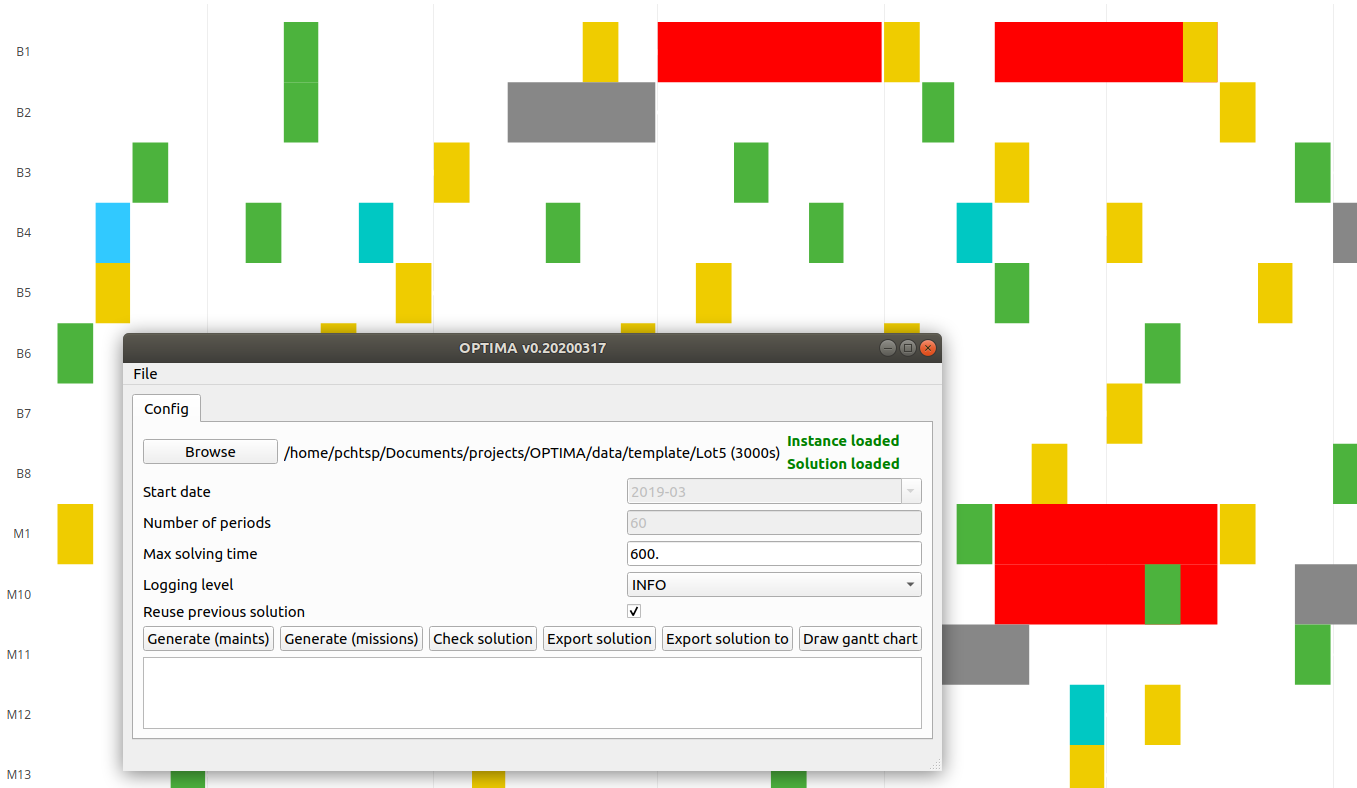
\includegraphics[width=0.9\linewidth]{images/gantt_solution_3.png}
%   % }
%   % \only<2>{  
%   %   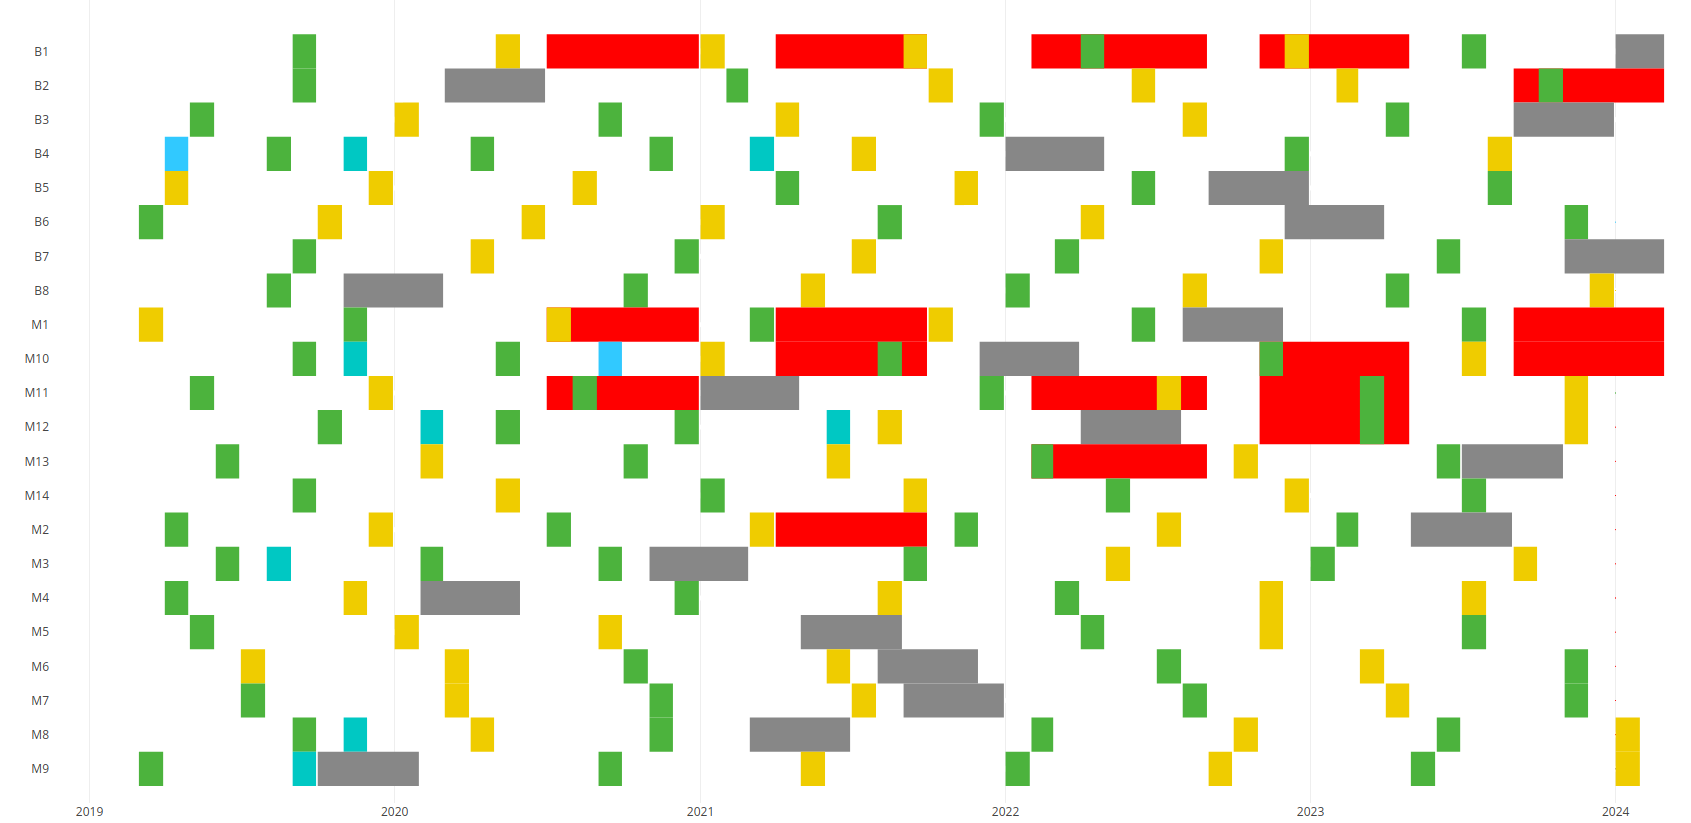
\includegraphics[width=0.8\linewidth]{images/gantt_solution.png}
%   % }

% \end{frame}

\begin{frame}
\frametitle{\textbf{Perspectives}}
  % \end{block}  
  % \pause
  % \begin{block}{\textbf{Perspectives}}
    \begin{itemize}[<+->]
      \item \textbf{Extend the problem} to include some additional secondary constraints.        
      \item \textbf{Integrate} novel techniques (ML and graph) inside known frameworks (Column Generation, GRASP).
      \item \textbf{Generalize ML methodology}
        to obtain a probability distribution for patterns, automatize feature extraction.
      \item \textbf{Combine ML and VND},
        e.g., by applying learned-cuts during path-sampling to extract promising patterns.
    \end{itemize}
  % \end{block}
\end{frame}

\begin{frame}
\frametitle{\textbf{Contributions}}

\fontsize{6pt}{7.2}\selectfont
\begin{block}{\textbf{Journal articles}}

  \begin{itemize}
    \item F. Peschiera, R. Dell, J. Royset, A. Haït, N. Dupin, and O. Battaïa. A novel solution approach with ML-based pseudo-cuts for the Flight and Maintenance Planning problem. OR Spectrum, pages 1–30, jun 2020. ISSN 0171-6468. doi: 10.1007/s00291-020-00591-z.

    \item F. Peschiera, A. Haït, N. Dupin, and O. Battaïa. Long term planning of military aircraft flight and maintenance operations. Technical report, ISAE-SUPAERO, Université de Toulouse, France, 2020 (submitted).

    \item  F. Peschiera, N. Dupin, A. Haït, and O. Battaïa. Novel graph-based matheuristic to solve the flight and maintenance planning problem. Forthcoming (to be submitted).
  \end{itemize}

\end{block}

\begin{block}{\textbf{Conferences}}

  \begin{itemize}
    \item F. Peschiera, A. Haït, N. Dupin, and O. Battaïa. Maintenance planning on french military aircraft operations. In Congrès annuel de la société Française de Recherche Opérationnelle et d’Aide à la Décision (ROADEF), pages 1–2, Lorient, FR, 2018.

    \item F. Peschiera, O. Battaïa, A. Haït, and N. Dupin. Bi-objective mip formulation for the  optimization of maintenance planning on french military aircraft operations. 2018. 
    
    \item F. Peschiera, A. Haït, N. Dupin, and O. Battaïa. A novel mip formulation for the optimization problem of maintenance planning of military aircraft. In XIX Latin-Iberoamerican Conference on Operations Research, Lima, PE, 2018
    
    \item F. Peschiera, N. Dupin, O. Battaïa, and A. Haït. An alternative mip formulation for the military flight and maintenance planning problem. In Congrès annuel de la société Française de Recherche Opérationnelle et d’Aide à la Décision (ROADEF), Montpellier, FR, 2020.

  \end{itemize}
\end{block}

\end{frame}

% \begin{frame}
% \frametitle{\textbf{Congress presentations}}
% % \begin{block}{\textbf{}}

%   \begin{itemize}
%     \item F. Peschiera, A. Haït, N. Dupin, and O. Battaïa. Maintenance planning on french military aircraft operations. In Congrès annuel de la société Française de Recherche Opérationnelle et d’Aide à la Décision (ROADEF), pages 1–2, Lorient, FR, 2018.

%     \item F. Peschiera, O. Battaïa, A. Haït, and N. Dupin. Bi-objective mip formulation for the  optimization of maintenance planning on french military aircraft operations. 2018. 
    
%     \item F. Peschiera, A. Haït, N. Dupin, and O. Battaïa. A novel mip formulation for the optimization problem of maintenance planning of military aircraft. In XIX Latin-Iberoamerican Conference on Operations Research, Lima, PE, 2018
    
%     \item F. Peschiera, N. Dupin, O. Battaïa, and A. Haït. An alternative mip formulation for the military flight and maintenance planning problem. In Congrès annuel de la société Française de Recherche Opérationnelle et d’Aide à la Décision (ROADEF), Montpellier, FR, 2020.

%   \end{itemize}
% % \end{block}

% \end{frame}

